\chapter{The physical layout}
\label{cha:PHYLAY}\index{Physical layout}
This chapter explores the physical storage. We'll start from the data files 
moving deep into the data blocks and finally to the tuples.  After looking to 
the tablespaces we'll complete the outline started in \ref{sec:TRANSACTION} 
with the MVCC\index{MVCC}.

\section{Data files}\index{Data files}
Wherever the database stores the files, the \$PGDATA/base or a different 
tablespace, those files are named, initially, after the relation's object 
identifier, a 4 byte unsigned integer. The word \textit{initially} means 
there's no guarantee the file will stay the same in the future.
Some file altering operations like the REINDEX or the VACUUM FULL change the 
file name leaving the relation's object identifier unchanged.

The maximum size allowed for a datafile is 1 GB, then a new segment with 
the same name and a sequential suffix is created. 
For example if the relation 34554001 reaches the upper limit a new file named 
34554001.1 is added, when this one reaches 1 GB then a 34554001.2 is added and 
so on. 

Alongside the main data files there're some additional forks needed for the 
database activity.

\subsection{Free space map}\index{Free space map}
The free space map segment is present for the index\index{Index, files} and 
table's data files . It's named after the relation's filenode with the suffix 
\_fsm and is used to track the free space in the relation. 

\subsection{Visibility map}\index{Visibility map}
The table's file are also called heap files\index{Heap, files}. Alongside those 
files there is a second fork called visibility map. Like before this file 
is named after the relation's filenode with the suffix \_vm.
Its usage is  for tracking the data pages  having all the tuples visible to all 
the active transactions. This fork is used also for the index only 
scans\index{index only scans} where the data is retrieved from the index page 
only.

\subsection{Initialisation fork}\index{Initialisation fork}
The initialisation fork is an empty table or index page, stored alongside the 
unlogged relation's data file. As seen in \ref{sub:UNLOGGEDTABLES} when the 
database performs a crash recovery the unlogged relations are zeroed. The 
initialisation fork is used to reset them and all the relation's accessory 
forks are deleted.

\subsection{pg\_class}
All the current database's relations are listed in the 
pg\_class\index{pg\_class} system table. The 
field relfilenode shows the relation's filename. \newline

The oid field, hidden if wildcard is used in the select list, is the internal 
object identifier. 
PostgreSQL is shipped with plenty of useful functions to get informations from 
the relation's OID. For example the function 
pg\_total\_relation\_size(regclass) returns the space used by the 
table plus the indices, the additional forks and the eventual TOAST table.
The function returns the size bytes. Another function, the 
pg\_size\_pretty(bigint), returns a human readable format for better 
reading.\newline

The field relkind is used to track the relation's kind

\begin{table}[h]
  \begin{tabular}{cc}
    Value & Relation's kind 
Read\\ 
    \hline
    r  &  ordinary table \\
    i  &  index \\
    S  &  sequence \\
    v  &  view \\
    m  &  materialised view \\
    c  &  composite type \\
    t  &  TOAST table \\
    f  &  foreign table \\
    
  \end{tabular}
  \caption{\label{tab:RELKIND}Relkind possible values}
\end{table}

\section{Pages}\index{Data pages}
The datafiles are organized as array of fixed length elements called pages. The 
default size is 8k. Pages of a table's datafile are called heap 
pages\index{Heap pages} to distinguish from the index pages\index{Index pages} 
which differs from the former only for the special space present in the page's 
end. The figure \ref{fig:INDEX01} shows an index page structure. The special 
space is small area in the page's end used to track down the index structure. 
For example a B-tree index stores in the special space the pointers to the leaf 
pages.

\begin{figure}[H]
\begin{center}

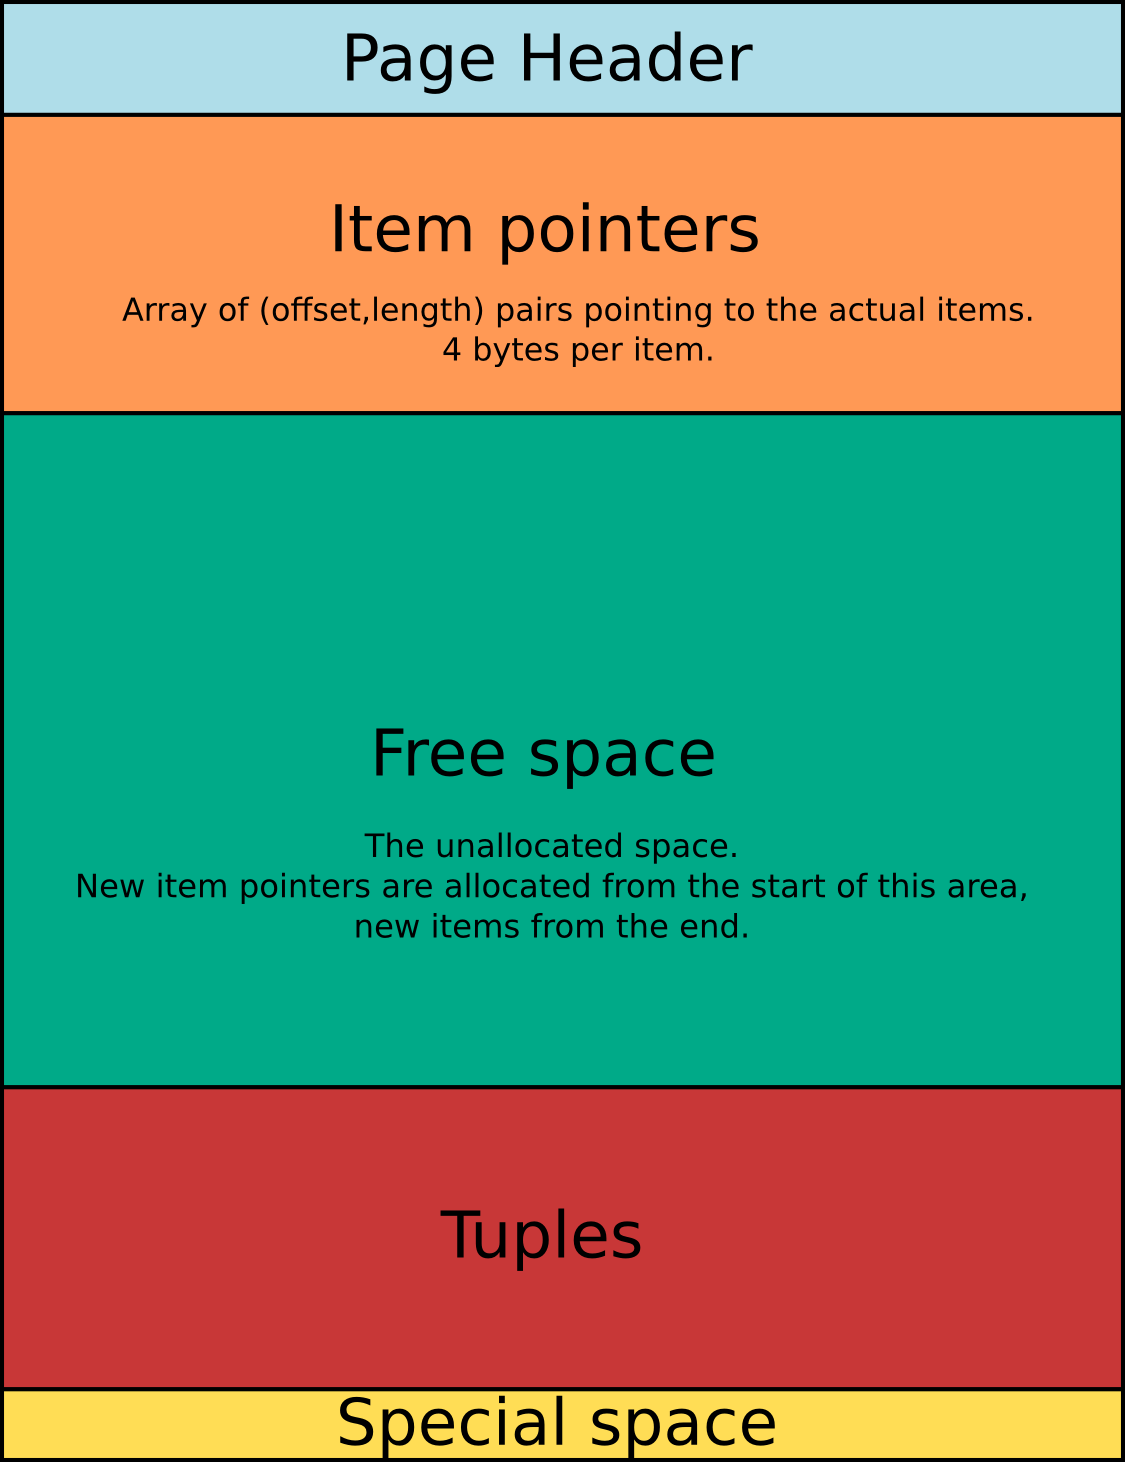
\includegraphics[scale=0.35]{images/index_page_01.png}

\caption{Index page}
\label{fig:INDEX01} 
\end{center}

\end{figure}

The page starts with a header \index{Data pages,header}24 bytes long followed 
by 
the item pointers, usually 4 bytes long. In the page's bottom are stored the 
actual items, the tuples.\newline

The item pointers\index{Item pointers} is an array of pairs, offset and 
length, pointing the actual tuples in the page's bottom. The tuples are put in 
the page's bottom and going backwards to fill up all the available free 
space.\newline 

The header contains the page's generic space management informations as shown 
in figure \ref{fig:HEADERPAG01}. 


\begin{figure}[H]
\begin{center}

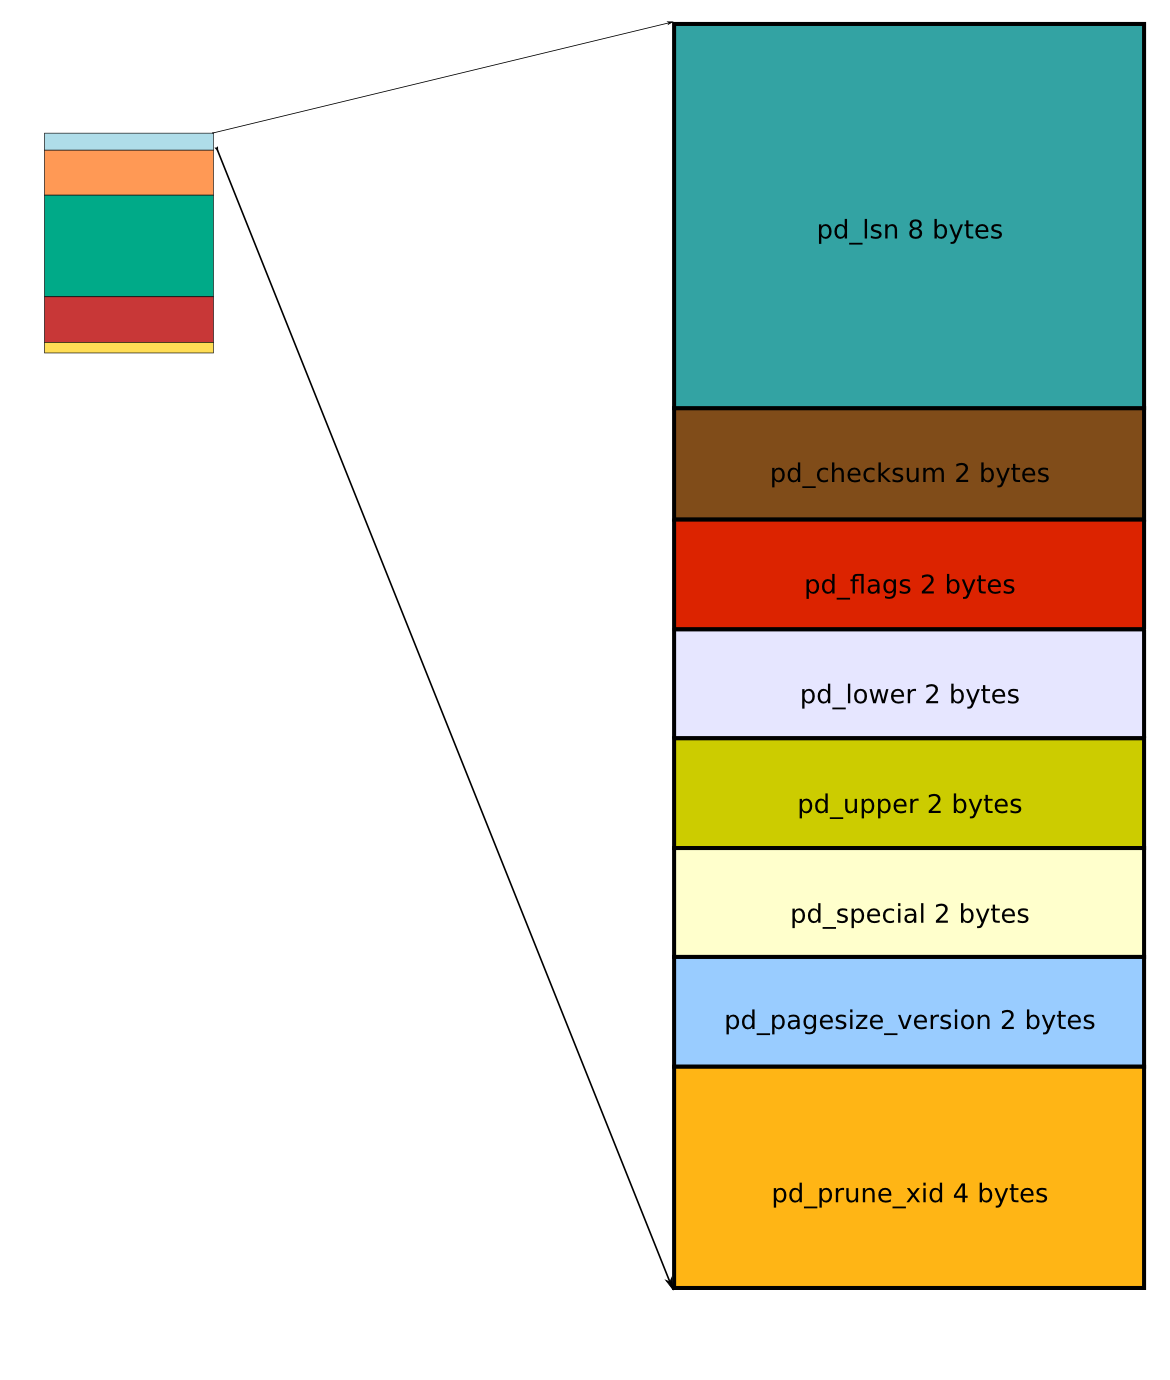
\includegraphics[scale=0.55]{images/header_page_01.png}

\caption{Page header}
\label{fig:HEADERPAG01} 
\end{center}

\end{figure}
\begin{itemize}
 \item \textbf{pd\_lsn} identifies the xlog record for last page's change.  The 
buffer manager uses the  LSN for WAL enforcement. A dirty buffer is not dumped 
to the disk until the xlog has been flushed at least as far as the page's LSN.
\item \textbf{pd\_checksum} stores the page's checksum if enabled, otherwise 
this field remain unused
\item \textbf{pd\_flags} used to store the page's flags 
\item \textbf{pg\_lower} offset to the start of the free space
\item \textbf{pg\_upper} offset to the end of the free space
\item \textbf{pg\_special} offset to the start of special space
\item \textbf{pd\_pagesize\_version} page size and page version packed 
together in a single field. 
\item \textbf{pg\_prune\_xid} is a hint field to helpt to determine if pruning 
is useful.  It's used only on the heap pages.

\end{itemize}

The pd\_checksum \index{Page checksum}field substitute the pd\_tli field 
present in the page header up to PostgreSQL 9.2 and used to track the 
xlog record across the timeline id. 
The page's checksum can be enabled only when the data area is initialised with 
initdb and cannot be disabled later.\newline

The offset fields, pg\_lower, pd\_upper and the optional pd\_special, are 2 
bytes long, this means PostgreSQL can only support pages up to 32KB.\newline

The page version\index{Page version} was introduced with PostgreSQL 7.3. 
For the prior releases the page version is arbitrarily considered 0; PostgreSQL 
7.3 and 7.4 had the page version to 1; PostgreSQL 8.0 used the version 2; 
PostgreSQL 8.1 and 8.2 used version number 3; From PostgreSQL 8.3 the page's 
version number is 4.

\section{Tuples}\index{Tuples}
\label{sec:TUPLES}
As seen in \ref{sec:TRANSACTION} PostgreSQL when updating the rows, generates 
new row versions stamping the old as dead. \newline

Each tuple comes with a fixed header of system columns usually 23 bytes as 
shown in the figure \ref{fig:TUPLES01}.\newline





\begin{figure}[H]
\begin{center}

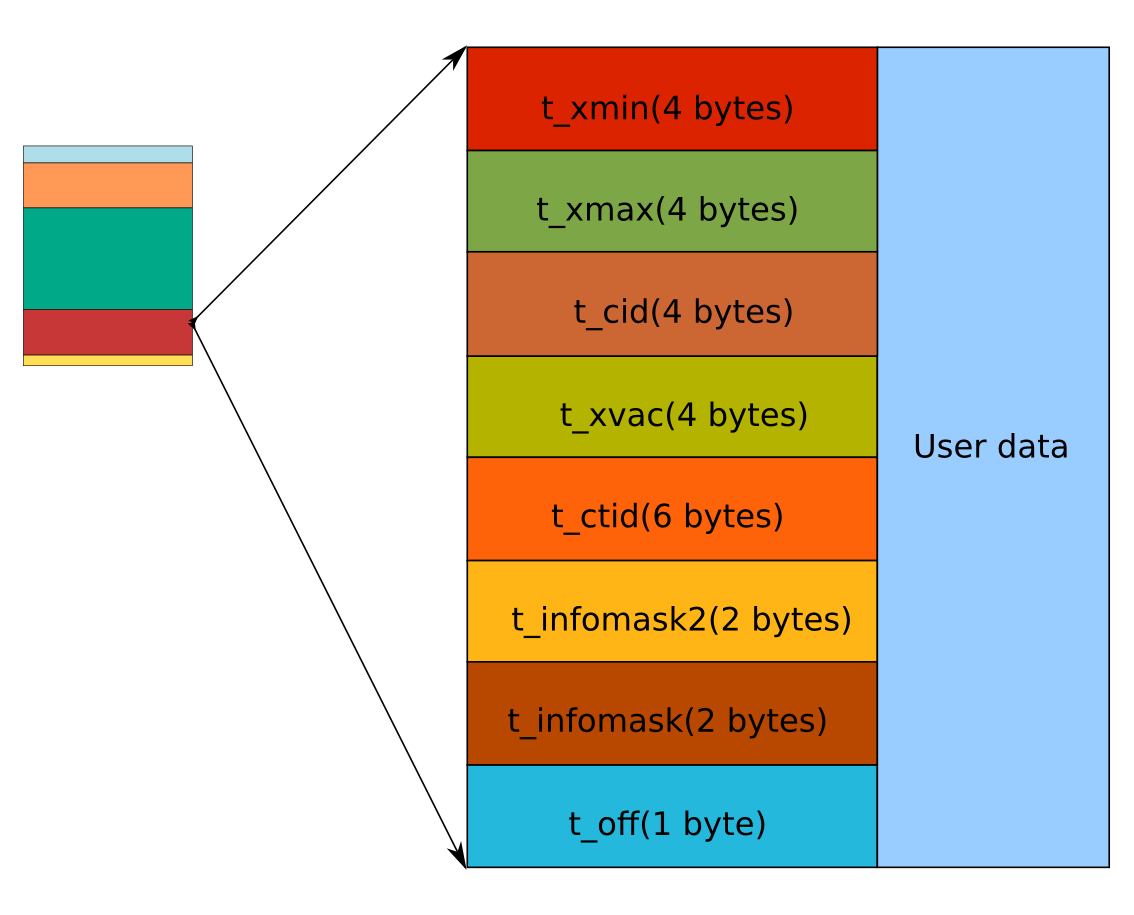
\includegraphics[scale=0.55]{images/tuples_01.png}

\caption{Tuple structure}
\label{fig:TUPLES01} 
\end{center}

\end{figure}

The two fields t\_xmin\index{t\_xmin} and t\_xmax\index{t\_xmax} are stamped 
respectively at tuple's insert and delete with the operation's transaction 
id.\newline 

The field t\_cid\index{t\_cid} is a ``virtual'' field used either for cmin and 
cmax. This is 
possible because the command id have meaning only inside a transaction.\newline

The field t\_xvac\index{t\_xvac} is used by VACUUM when moving the rows, 
according with the source code's comments in src/include/access/htup\_details.h 
this is used only by old style VACUUM FULL. \newline

The t\_cid\index{t\_cid} is the tuple's location id, a couple of integers 
pointing the page number and the tuple's index. When a new tuple is created 
t\_cid is set to the actual row's value; When the tuple is updated the this 
value changes to the location of the newer tuple's version. \newline

A tuple is then recognised as last version when xmax is invalid or t\_cid 
points to itself. If xmax is also valid then the tuple is the last locked or 
deleted version of the tuple's version chain.\newline

The two infomask fields are used to store various flags like the presence of the tuple OID or if 
the 
tuple has NULL values.\newline
The last field t\_off is used to mark the offset to the composite data, the actual tuple's data. 
This field's value is usually zero if the table doesn't have NULLable fields or is created WITH 
OIDS. If present, tThe OID and the a NULL bitmap are placed just after the tuple's header. The 
bitmap begins just after the fixed header and occupies enough bytes to have one bit per data 
column. 
The OID comes after the bitmap and is 4 bytes long.


\section{TOAST}\index{TOAST}
\label{sec:TOAST}
The oversize attribute storage technique is the PostgreSQL implementation for the data overflowing 
the page size.\newline

The user data shown in figure \ref{fig:TUPLES01} is a stream of composite data. Actually the data 
itself is logically described by the composite model stored in the system catalogue. The attributes 
in the model can be grouped in two categories, the fixed length and the variable length data type 
(varlena).\newline

For example, a four bytes integer is a fixed length type and a text is a variable length. For the 
PostgreSQL's internal routines the data at physical level appears all the same, as a generic datum. 
When the datum\index{datum} is loaded into the shared buffer becomes meaningful and is managed 
accordingly with its nature.\newline

The attribute's kind is stored in the first two bits\footnote{On the big-endian architecture those 
are the high-order bits; on the little-endian those are the low-order bits} of the 
varlena\index{varlena} length word. When both bits are zero then the attribute is a fixed length 
data type and the remaining bits give the datum size in bytes including the length word.\newline

If the first bit is set then the value have only a single-byte header and the remaining bits 
describe the total datum size in bytes including the length byte. If the remaining bits are all 
zero, then the value is a pointer to an out of line data stored in a separate TOAST table which 
structure is shown in figure \ref{fig:TOAST01}.\newline

If the first bit is zero but the second bit is set then the datum is compressed and must be 
decompressed before the use. The compression uses the LZ family algorithm.\newline

the OID of the toasted data, the chunk\_seq and integer for ordering the chunks 
within the value and the chunk\_data, a bytea field containing the the 
overflown data.\newline 

The chunk size is normally 2k and is controlled at compile time by the symbol 
TOAST\_MAX\_CHUNK\_SIZE. The TOAST code is triggered by the value TOAST\_TUPLE\_THRESHOLD, also 2k 
by default. When the tuple's size is bigger then the TOAST routines are triggered.\newline

The TOAST\_TUPLE\_TARGET normally 2 kB as well governs the compression's behaviour. PostgreSQL will 
compress the datum to achieve a final size lesser than TOAST\_TUPLE\_TARGET. If cannot then the out 
of line storage is used.

\begin{figure}[H]
\begin{center}

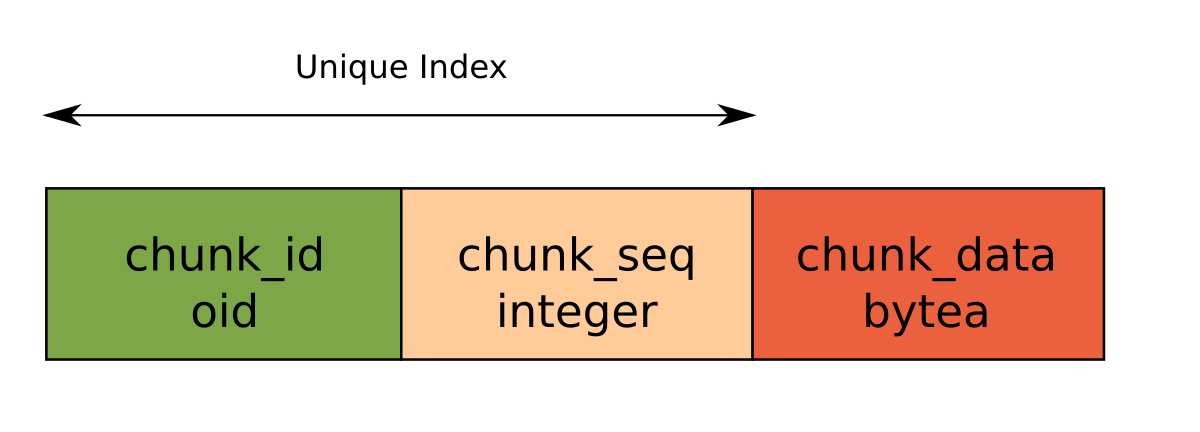
\includegraphics[scale=0.55]{images/toast_01.png}

\caption{Toast table structure}
\label{fig:TOAST01} 
\end{center}

\end{figure}

TOAST offers four different storage strategies. Each strategy can be changed per column using the  
ALTER TABLE SET STORAGE statement.
\begin{itemize}
 


\index{TOAST, storage strategies}
\item     PLAIN prevents either compression or out-of-line storage; It's the only storage available 
for fixed length data types.

\item     EXTENDED allows both compression and out-of-line storage. It is the default for most 
TOAST-able data types. Compression will be attempted first, then out-of-line storage if the row is 
still too big.

\item     EXTERNAL allows out-of-line storage but not compression. 

\item     MAIN allows compression but not out-of-line storage. Actually the out-of-line storage is 
still performed as last resort.

\end{itemize}

The out of line storage\index{TOAST, out of line storage} have the advantage of leaving out the 
stored data from the row versioning; if the TOAST data is not affected by the update there will be 
no dead row for the TOAST data. That's possible because the varlena is a mere pointer to the chunks 
and a new row version will affect only the pointer leaving the TOAST data unchanged.\newline
The TOAST table are stored like all the other relation's in the pg\_class table, the associated 
table can be found using a self join on the field reltoastrelid.\newline

Because the TOAST usurps two bits in the varlena length word, this limits the maximum allocated 
size 
for the datum to 1GB \begin{math} (2^{30} -1 bytes) \end{math} .

\section{Tablespaces}\index{tablespaces,physical}
\label{sub:TBS-PHYSICAL}
PostgreSQL implements the tablespaces creating the symbolic links, pointing the tablespace's 
location, into the pg\_tblspc. The links are named like the tablespace's OID. The tablespaces are 
available only on systems supporting the symbolic links.\newline

Since PostgreSQL 9.1 the tablespace location was stored into the field spclocation of the 
pg\_tablespace\index{pg\_tablespace} system table. The information was used only to dump the 
tablespace's definition during a pg\_dump and was removed in the version 9.2 and it was was 
introduced the function pg\_tablespace\_location(tablespace\_oid) to get the tablespace's absolute 
path from the tablespace oid.\newline

Querying the system catalogue to acquire any sort of informations is quite  simple. In this example 
the query returns the tablespace's location seen in \ref{sub:TBS-LOGICAL} 

\begin{lstlisting}[style=pgsql]
 postgres=# 
 SELECT 
        pg_tablespace_location(oid),
        spcname 
FROM 
        pg_tablespace;
       pg_tablespace_location       |  spcname   
------------------------------------+------------
                                    | pg_default
                                    | pg_global
 /var/lib/postgresql/pg_tbs/ts_test | ts_test
(3 rows)

\end{lstlisting}

The function returns the empty string for the system tablespaces, pg\_default and pg\_global, 
because those locations have an immutable location, relative to the data directory. We can get the 
data area's absolute path using the function current\_settings. 

\begin{lstlisting}[style=pgsql]
 postgres=# SELECT current_setting('data_directory');
       current_setting        
------------------------------
 /var/lib/postgresql/9.3/main
(1 row)

\end{lstlisting}

Using the CASE construct is then possible to build up an more complete query to lookout at the 
tablespaces locations.\newpage

\begin{lstlisting}[style=pgsql]
 postgres=# 
SELECT 
        CASE
                WHEN 
                                pg_tablespace_location(oid)=''
                        AND     spcname='pg_default'
                THEN
                        current_setting('data_directory')||'/base/'
                WHEN 
                                pg_tablespace_location(oid)=''
                        AND     spcname='pg_global'
                THEN
                        current_setting('data_directory')||'/global/'
        ELSE
                pg_tablespace_location(oid)
        END
        AS      spclocation,
                
        spcname 
FROM 
        pg_tablespace;
             spclocation              |  spcname   
--------------------------------------+------------
 /var/lib/postgresql/9.3/main/base/   | pg_default
 /var/lib/postgresql/9.3/main/global/ | pg_global
 /var/lib/postgresql/pg_tbs/ts_test   | ts_test
(3 rows)

\end{lstlisting}

Before the version 8.4 the tablespace location pointed directly to the referenced directory, 
causing 
a potential location's clash. The newer versions introduced the usage of a container directory into 
the tablespace location named after the major version and the system catalogue version number. 
\newline

\begin{verbatim}

postgres@tardis:~$ ls -l /var/lib/postgresql/pg_tbs/ts_test
total 0
drwx------ 2 postgres postgres 6 Jun  9 13:01 PG_9.3_201306121

\end{verbatim}

The tablespace's directory container is structured this way\newline
PG\_\{MAJOR\_VERSION\}\_\{CATALOGUE\_VERSION\_NUMBER\}\newline

The major version is the PostgreSQL version truncated to the second cypher and the catalogue's 
version number is the same shown in the pg\_controldata output, a formatted date.

\begin{verbatim}
postgres@tardis:~$ export PGDATA=/var/lib/postgresql/9.3/main
postgres@tardis:~$ /usr/lib/postgresql/9.3/bin/pg_controldata 
pg_control version number:            937
Catalog version number:               201306121
Database system identifier:           5992975355079285751
Database cluster state:               in production
pg_control last modified:             Mon 09 Jun 2014 13:05:14 UTC
.
.
.
WAL block size:                       8192
Bytes per WAL segment:                16777216
Maximum length of identifiers:        64
Maximum columns in an index:          32
Maximum size of a TOAST chunk:        1996
Date/time type storage:               64-bit integers
Float4 argument passing:              by value
Float8 argument passing:              by value
Data page checksum version:           0

\end{verbatim}

Inside the container directory the structure is same as the directory base seen in 
\ref{sec:PGDATA}, 
with one difference. There're only the subdirectories for the databases having relations on the 
tablespace.\newline

To get all the databases with objects on the current tablespace it's present the function 
pg\_tablespace\_databases(tablespace\_oid) which returns the set of the database OID with objects 
on 
the specified tablespace. In order to have a better picture we can join the query with the 
pg\_database system table.\newline

Here's an example query using the CASE construct with the pg\_tablespace\_databases function, to 
get 
all the databases with objects on the ts\_test tablespace.\newpage
\begin{lstlisting}[style=pgsql]
 db_test=# 
 SELECT
        datname,
        spcname,
        CASE
                WHEN 
                                pg_tablespace_location(tbsoid)=''
                        AND     spcname='pg_default'
                THEN
                        current_setting('data_directory')||'/base/'
                WHEN 
                                pg_tablespace_location(tbsoid)=''
                        AND     spcname='pg_global'
                THEN
                        current_setting('data_directory')||'/global/'
        ELSE
                pg_tablespace_location(tbsoid)
        END
        AS      spclocation
FROM
        pg_database dat,
        (
                SELECT
                        oid as tbsoid,
                        pg_tablespace_databases(oid) as datoid,
                        spcname 
                FROM 
                        pg_tablespace where spcname='ts_test'
        ) tbs
WHERE
        dat.oid=tbs.datoid
;
 datname | spcname |            spclocation             
---------+---------+------------------------------------
 db_test | ts_test | /var/lib/postgresql/pg_tbs/ts_test
(1 row)

\end{lstlisting}

Moving a tablespace to another physical location it's not complicated; the cluster of course has to 
be shut down; see \ref{sec:SHUTDOWN_SEQ} for more informations about the shutdown sequence.\newline

When the cluster is stopped the container directory can be copied to the new location; the 
directory's access permissions must be the same as the origin; read write for the os user running 
the postgresql process only, otherwise the cluster will refuse to start.\newline

When the copy is complete and the symbolic link in \$PGDATA/pg\_tblspc is fixed to point the new 
location the cluster can be started as shown in \ref{sec:STARTUP}.

\section{MVCC} \label{sec:MVCC}\index{MVCC} 
The multiversion concurrency control is the access method used by PostgreSQL to provide the 
transactional model as seen in \ref{sec:TRANSACTION}.\newline

At logical level this is completely transparent to the user and the new row versions become visible 
after the commit, accordingly with the transaction isolation level. \newline

At physical level we have for each new row version, the insert's XID stamped into the t\_xmin 
field. The PostgreSQL's internal semantic makes visible only the committed rows stamped with the 
XID lesser than the current transaction's XID because considered \textit{in the past}. The rows 
with 
a XID greater than the current transaction's XID are considered \textit{in the future} and then 
invisible.\newline

Because the XID is a 32 bit quantity, it wraps at 4 billions. When this happens theoretically all 
the tuples should suddenly disappear because they switch from in the XID's past to its future. This 
is the XID wraparound failure,\index{XID wraparound failure} a serious problem for the older 
PostgreSQL versions, which only fix was to re init a new data area each 4 billion transactions and 
dump reload the databases.\newline 

PostgreSQL 7.2 introduced the \begin{math}modulo-2^{32}\end{math} arithmetic for evaulating the XID 
age where a special XID, the FrozenXID\footnote{The FrozenXID's value is 2. The docs of PostgreSQL 
7.2 also mention the BootstrapXID with value 1} was assumed as always in the past and having, for 
any given XID 2 billion transactions in the future and 2 billion transactions in the past.\newline

When the age of the stamped t\_xmin becomes old then the VACUUM\index{VACUUM} can freeze 
the tuple stamping the FrozenXID and preserving it from the disappearance. The pg\_class and the 
pg\_database table have a dedicated field to track the oldest tuple inside the relation and the 
database, respectively the relfrozenxid  and the datfrozenxid where the oldest not frozen XID's 
value is stored. The builtin function age() shows how many transactions are between 
the current XID and the value stored in the system catalogue. \newline

For example this is a query to get all the databases with the datfrozenxid and the age.\newpage

\begin{lstlisting}[style=pgsql]
 postgres=# 
        SELECT 
                datname,
                age(datfrozenxid),
                datfrozenxid 
        FROM 
                pg_database;
    datname    | age  | datfrozenxid 
---------------+------+--------------
 template1     | 4211 |          679
 template0     | 4211 |          679
 postgres      | 4211 |          679
 db_test       | 4211 |          679

\end{lstlisting}

The datfroxenxid value is meaningful only through the age function which shows the
``distance'' between the current XID and the datfroxenxid. PostgreSQL assigns the new 
XID only for the write transactions and only if the tuples are updated in the so called ``lazy XID 
assignment''.\newline 


When a tuple's XID becomes older than 2 billion transactions, the tuple simply disappears  jumping 
from the the current XID's past to its future. Before the version 8.0 there was no prevention
for this problem, except the periodic cluster wide VACUUM. The latest versions introduced a 
passive protection mechanism emitting messages in the activity log when the age of datfrozenxid is  
ten million transactions from the wraparound point.

\begin{smallverbatim}
WARNING:  database "test_db" must be vacuumed within 152405486 transactions
HINT:  To avoid a database shutdown, execute a database-wide VACUUM in 
"test_db".
\end{smallverbatim}

Another active protection is the autovacuum daemon which take care of the affected tables and 
starts a VACUUM to freeze the tuples even  if autovacuum is turned off. However if something goes 
wrong and the datfrozenxid reaches one million transactions from the wraparound point, the 
cluster shutdown and keeps shutting down for each transaction. When this happens the cluster 
can be only  started in single-user backend to execute the VACUUM.\newline

To limit the effect of data bloat, unavoidable with this implementation,  PostgreSQL have the 
feature called HOT\index{HOT strategy} which stands for Heap Only Tuples. The RDBMS tries to keep 
the updated tuples inside the same page avoiding also any index reference update, if present. This 
is possible only if there's available free space. By default PostgreSQL when inserting the 
tuples, fills up the pages completely; however is possible to reserve a page portion for the 
updates with the fillfactor storage parameter\index{fillfactor storage parameter}. This is the 
percentage of the page to reserve for the inserts. The default value for the heap pages is 100, 
complete packing. For the indices is 70 for the not leaf pages and 90 for the leaf pages leaving 
some space available for the unavoidable updates. A smaller fill factor will result, at insert time, 
with a bigger table but with lesser grow rate when updated. \newline

Finally if the MVCC is not carefully considered at design time, this can result in data bloat and 
generally poor performances.
In the \ref{cha:MAINTENANCE} we'll see how and how to keep the cluster in efficient conditions or 
at least how to try.